\subsection{Bitcoind}
\label{sec:bitcoind}
Il primo componetene del sistema distribuito ha il compito di fornire i dati da elaborare. Questa funzione è svolta dal demone Bitcoind.
\\Bitcoind, formalmente, è un software che implementa il protocollo Bitcoin per l'utilizzo delle remote procedure call (RPC). Esso è anche il secondo client Bitcoin nella storia del network \cite{wiki:bitcoind}. Per sua natura, è eseguito come processo in background quindi l'utente per interagire con esso ha bisogno di farlo tramite una interfaccia da riga di comando chiamata \textit{bitcoin-cli}. Il demone, inoltre, funge da nodo della rete Bitcoin, infatti si sincronizza con la blockchain, verifica le transazioni ed invia blocchi. Esiste una versione anche con interfaccia grafica del demone chiamata \textit{Bitcoin-QT o Bitcoin Core}, ma per lo scopo dell'elaborato si è preferito utilizzare la versione lite per limitare l'utilizzo di risorse.
\\La versione demone, inoltre, ha il vantaggio di creare una coda ZeroMQ per la comunicazione con applicazioni esterne. Il sistema distribuito, utilizza questa funzione per recuperare i blocchi in formato grezzo (sequenza di byte) ogni qualvolta sono validati dalla blockchain.

\subsubsection{ZeroMQ}
\label{sec:ZMQ}
ZeroMQ (anche conosciuto come ØMQ, 0MQ, o zmq) è una libreria di messagistica asincrona ad alte prestazioni, destinata all'uso in applicazioni distribuite o concorrenti. Fornisce code di messaggi, ma a differenza dei middleware orientati ai messaggi, il sistema ZeroMQ può essere eseguito senza un broker di messaggi dedicato \cite{wiki:ZMQ}. La libreria, inoltre, funziona molto bene grazie al suo modello interno di threading, che può superare le tradizionali applicazioni TCP in termini di throughput utilizzando una tecnica di batching automatico dei messaggi \cite{ZMQ-throughput}. Il suo modello I/O asincrono offre la possibilità di creare applicazioni multicore scalabili, costruite come attività asincrone di elaborazione dei messaggi. Inoltre, la comunità di sviluppatori, ha creato una quantità enorme di wrapper per la libreria, così da renderla funzionante sulla maggior parte dei sistemi operativi. All'interno del sistema distribuito, infatti, è stato utilizzato il wrapper \textit{jzmq} che permette l'utilizzo della libreria tramite Java API. 
\\ZMQ, può avere diverse modalità di invio di messaggi atomici:
\begin{itemize}
\item Request-reply: Connette un insieme di clienti ad un insieme di servizi. Questo è una Remote Procedure Call (RPC).
\item Publish-subscribe: Connette un insieme di produttori ad un insieme di consumatori.
\item Push-pull (pipeline): Connette i nodi in un pattern fan-out/fan-in che può avere più passaggi e cicli. Distribuisce in maniera parallela i messaggi.
\item Exclusive pair: Collega due socket in maniera esclusiva.
\end{itemize}
Bitcoind utilizza una socket di tipo Publish-subscribe. Il publisher, in questo caso bitcoind, può spedire un messaggio a molti consumers attraverso un canale virtuale chiamato topic. Uno stesso topic può essere condiviso da più subscriber (client). Per ricevere i messaggi, i client devono "sottoscriversi" al topic creato da bitcoind. Ovviamente, questo implica che c'è relazione temporale tra i publisher e i subscibers, nel senso che, un client che si sottoscrive ad un topic può consumare solamente i messaggi pubblicati dopo la sua sottoscrizione.  Qualsiasi messaggio spedito sul topic, viene consegnato a tutti i consumer sottoscritti, ciascuno dei quali riceve una copia identica di ciascun messaggio inviato. I messaggi quindi, vengono automaticamente inviati in broadcast ai consumer, senza che questi ne abbiano fatto esplicita richiesta.
\\Nel caso del sistema distribuito, il client che si sottoscrive al topic \textit{pubrawblock} di bitcoind è il connettore-subscriber implementato all'interno di Spark. 
\begin{figure}[H]
	\centering
	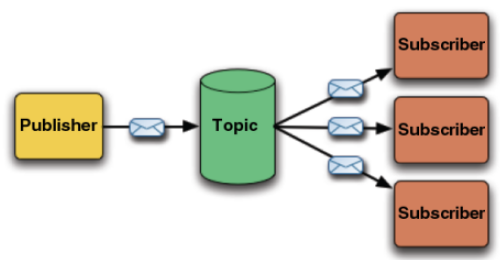
\includegraphics[width=\textwidth, height=0.25\textheight, keepaspectratio]{images/sub_pub.png}
	\caption{Messaggio inviato con la modalità Publish-Subscribe.}
	\label{fig:PubSubTopic}
\end{figure}